%* 
%* ------------------------------------------------------------------
%* CameraManual.tex - Manual for AnyDistance and Closest
%* Created by Robert Heller on Thu Mar 20 09:08:37 2008
%* ------------------------------------------------------------------
%* Modification History: $Log$
%* Modification History: Revision 1.1  2002/07/28 14:03:50  heller
%* Modification History: Add it copyright notice headers
%* Modification History:
%* ------------------------------------------------------------------
%* Contents:
%* ------------------------------------------------------------------
%*  
%*     Model RR System, Version 2
%*     Copyright (C) 1994,1995,2002-2005  Robert Heller D/B/A Deepwoods Software
%* 			51 Locke Hill Road
%* 			Wendell, MA 01379-9728
%* 
%*     This program is free software; you can redistribute it and/or modify
%*     it under the terms of the GNU General Public License as published by
%*     the Free Software Foundation; either version 2 of the License, or
%*     (at your option) any later version.
%* 
%*     This program is distributed in the hope that it will be useful,
%*     but WITHOUT ANY WARRANTY; without even the implied warranty of
%*     MERCHANTABILITY or FITNESS FOR A PARTICULAR PURPOSE.  See the
%*     GNU General Public License for more details.
%* 
%*     You should have received a copy of the GNU General Public License
%*     along with this program; if not, write to the Free Software
%*     Foundation, Inc., 675 Mass Ave, Cambridge, MA 02139, USA.
%* 
%*  
%* 


\chapter{Camera Programs Reference}
\label{chpt:camera:Reference}
\typeout{$Id$}

AnyDistance and Closest compute the view angle in both real and scale
units. It also computes the effective scale of the imaging plane, such
as the size of a 35mm slide, which might be used as a transparency for
model window panes or locomotive number boards.

Both programs work the same. The only difference is that Closest uses
the closest effective focus of the lens and AnyDistance uses a user
specificed focus distance.  Given the input parameters, the distance,
the lens, the scale, and the film size, a diagram is displayed with the
dimensions of the view.  This diagram can be printed using the \verb=Print...=
menu item under the \verb=File= menu.

New lenses can be entered with the \verb=New= menu item under the
\verb=File= menu. The \verb=Open...= and \verb=Save..= menu items can
load and save the set of available lenses.

Both programs solve Equation~\ref{eq:camera:viewWidth} and display a
diagram illustrating the solution.  AnyDistance uses a user entered
value for $D$ and Closest uses the closest focusing distance for the
selected lens.

\begin{equation}
W_{view} = (D S) 2 \tan(\frac{\theta}{2}) \label{eq:camera:viewWidth}
\end{equation}

Where:

\begin{eqnarray*}
W_{view} &=& \mbox{The scale view width.}\\
D &=& \mbox{The distance from the scene and the camera lens.}\\
S &=& \mbox{The model scale factor.}\\
\mbox{and} \\
\theta &=& \mbox{The lens view angle.}
\end{eqnarray*}

\begin{figure}[hbpt]
\begin{centering}
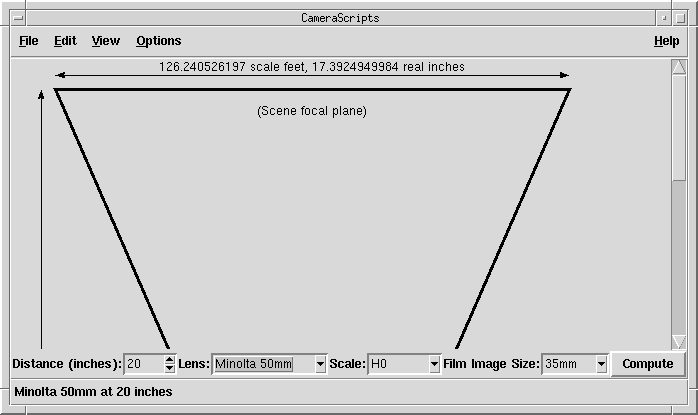
\includegraphics[width=5in]{CameraAnyDist.png}
\caption{The main GUI screen of the AnyDistance program}
\label{fig:camera:anydist}
\end{centering}
\end{figure}
The main GUI screen of the AnyDistance program is shown in
Figure~\ref{fig:camera:anydist}. The Closest program is much the same,
except that the distance parameter is ommited.
